\documentclass[aspectratio=1610]{beamer}
\usepackage[utf8]{inputenc}
\usepackage{amsmath, amssymb}

\title{Bezbedno izračunavanje sa više
učesnika}
\author{Marko Lazarević 1005/2025}
\date{\today}

\usetheme[color=nudarkblue,numbering=progressbar]{wildcat}

\begin{document}

\begin{frame}
\titlepage
\end{frame}

\begin{frame}{Sadržaj}
\tableofcontents

\end{frame}

\section{Uvod}
% ---------------- UVOD ----------------

\begin{frame}{Motivacija}
    \begin{itemize}
        \item Osnovni problem kriptografije: Bezbedan prenos poruka
        \item Difi-Helmanova razmena ključeva: 
        \begin{figure}[h]
            \centering
            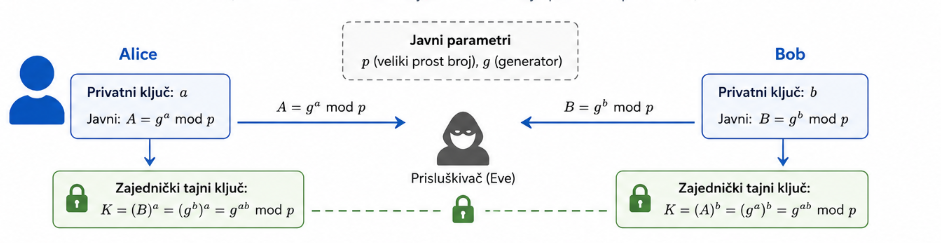
\includegraphics[width=\linewidth]{diffie_helman.png}
        \end{figure}

        \item Da li ovaj pristup možemo proširiti na opšte funkcije i više učesnika?
    \end{itemize}
\end{frame}


% ---------------- MPC DEFINICIJA ----------------
\begin{frame}{Bezbedno izračunavanje sa više učesnika}
\begin{pblock}{Definicija: MPC}
    \textbf{Bezbedno izračunavanje sa više učesnika} (eng. \textit{Secure Multi-Party Computation - MPC}) je oblast kriptografije koja se bavi problemom kako dva ili više učesnika mogu da izračunaju funkciju nad svojim privatnim ulazima, a da pritom ti ulazi ostanu privatni.
\end{pblock}
\begin{itemize}
    \item Idealni model: pouzdana treća strana koja neće otkriti ulaze
    \item Cilj: kreirati jednako siguran model bez treće strane 
\end{itemize}

\end{frame}

% ---------------- MILIONER PROBLEM ----------------
\begin{frame}{Problem milionera}

\begin{pblock}{Primer: Problem milionera}
    \begin{itemize}
        \item Više učesnika želi da sazna ko je najbogatiji
        \item Ne žele da otkriju vrednost svojih bogatstava
        \item Funkcija: indeks najbogatijeg učesnika
        \item MPC otkriva samo rezultat, ne i ulaze
        \item Koji podaci moraju biti otkriveni da bi se rešio problem?
    \end{itemize}
\end{pblock}
\end{frame}

% ---------------- MODELI PRETNJI ----------------
\begin{frame}{Modeli protivnika}
    \begin{itemize}
         \item \textbf{"Pošteni ali radoznali"} (eng. \textit{honest-but-curious}) protivnici - korektno izvršavaju protokol, ali pokušavaju da iz dostupnih informacija saznaju što više o privatnim podacima drugih učesnika
         \item \textbf{Zlonamerni} (eng. \textit{malicious}) protivnici - mogu proizvoljno odstupati od protokola i slati netačne podatke, pa protokol mora garantovati i privatnost i ispravnost izračunavanja
    \end{itemize}
\end{frame}

% ---------------- PRISTUPI ----------------
\begin{frame}{Osnovni pristupi MPC-u}
\begin{itemize}
    \item Šifrovana kola - Jaov protokol (eng. \textit{Yao's protocol})  zasnovan na šifrovanju funkcije kao binarnog kola, pogodan za dva učesnika
    \item Deljenje tajni - koristi aritmetička kola i savršeno sigurne šeme deljenja tajni, pogodan za više učesnika
\end{itemize}

\end{frame}

\section{Slučaj dva učesnika}
% ---------------- TWO PARTY ----------------
\begin{frame}{Slučaj dva učesnika}
\begin{itemize}
    \item Učesnici $A$ i $B$
    \item Privatni ulazi $x$ i $y$
    \item Cilj: izračunavanje zajedničke funkcije $f(x,y)$
    \item $A$ želi da sazna $f(x,y)$, ali ne želi da otkrije $x$
    \item $B$ želi da sazna $f(x,y)$, ali ne želi da otkrije $y$
\end{itemize}
\end{frame}

% ---------------- YAO IDEA ----------------
\begin{frame}{Jaov pristup}
\begin{itemize}
    \item Funkciju $f$ predstavlja kao binarno kolo
    \item Elementi kola su skup žica $W$ i skup logičkih kapija $G$
    \item Učesnik $A$ konstruše šifrovano kolo koje predstavlja funkciju $f$
    \item Učesnik $B$ evaluira šifrovano kolo i dobija rezultat $f(x,y)$ 
\end{itemize}
\end{frame}

% ---------------- CONSTRUCTION ----------------
\begin{frame}{Konstrukcija šifrovanog kola}
\begin{itemize}
    \item Za svaku žicu $w_i \in W$ se biraju dva nasumična kriptografska ključa, $k^0_i$ i $k^1_i$ za logičku nulu i logičku jedinicu.
    \item Za svaku žicu $w_i \in W$ definiše se njena logička vrednost $v_i \in \{0,1\}$ i bira se nasumična vrednost $\rho_i \in \{0, 1\}$ (permutacioni bit). Sa njom konstruišemo šifrovanu, ili ``spoljašnju'' vrednost, žice kao $e_i = v_i \oplus \rho_i$.
    \item Za svaku logičku kapiju $g_i \in G$ sa ulaznim žicama $w_{i_0}$ i $w_{i_1}$ i izlaznom žicom $w_{i_2}$, kreira se šifrovana tabela koja predstavlja funkciju kapije nad šifrovanim vrednostima žica. Za neku funkciju enkripcije sa dva ključa $E$, šifrovana tabela se satoji od vrednosti:
    \[
    c_{a,b}^{w_{i_2}} =
    E_{k_{w_{i_0}}^{a \oplus \rho_{i_0}},\,k_{w_{i_1}}^{b \oplus \rho_{i_1}}}
    \!\left(k_{w_{i_2}}^{o_{a,b}} \,\|\, (o_{a,b} \oplus \rho_{i_2})\right),
    \quad
    a,b\in\{0,1\}.
    \]
    gde je $o_{a,b}=g_i(a\oplus \rho_{i_0},\,b\oplus \rho_{i_1})$.
\end{itemize}
\end{frame}

\begin{frame}{Konstrukcija šifrovanog kola}
\begin{figure}[h]
    \centering
    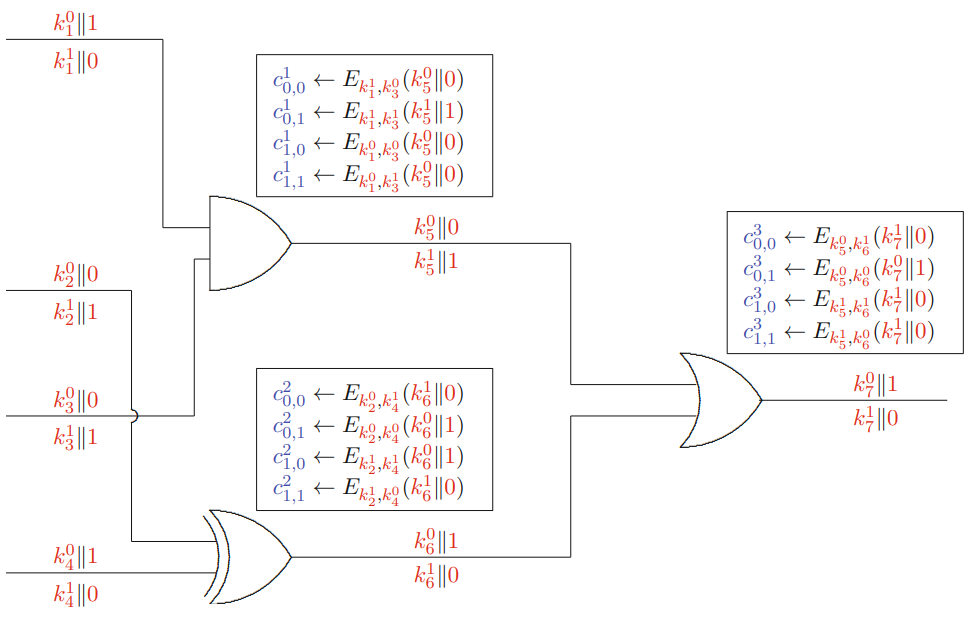
\includegraphics[width=0.8\linewidth]{garbled_1.png}
    \caption{Šifrovano kolo za $f(\{w_1,w_2\},\{w_3,w_4\})=(w_1\land w_3)\lor(w_2\oplus w_4)$.}
\end{figure}
\end{frame}
% ---------------- EVALUATION ----------------
\begin{frame}{Evaluacija šifrovanog kola}

\begin{itemize}
    \item Učesnik $B$ dobija šifrovanu tabelu
    \item Učesnik $A$ šalje $B$-u ključeve koji odgovaraju njegovim ulaznim vrednostima
    \item Učesnici $A$ i $B$ zatim izvršavaju protokol ignorantnog prenosa (eng. \textit{oblivious transfer, OT}) za svaku ulaznu žicu učesnika $B$ kako bi $B$ dobio tačno jedan od dva ključa koji odgovaraju njegovoj ulaznoj vrednosti
    \item Evaluacija se vrši tako što se kreće od ulaznih žica i koristi se šifrovana tabela da bi se dobile vrednosti izlaznih žica, sve dok se ne dođe do izlaza funkcije
    \item $B$ na kraju dobija šifrovanu vrednost izlazne žice, koju može dešifrovati koristeći $\rho$ vrednost izlazne žice da bi dobio rezultat $f(x,y)$
\end{itemize}

\end{frame}

\begin{frame}{Evaluacija šifrovanog kola}
\begin{figure}[h]
    \centering
    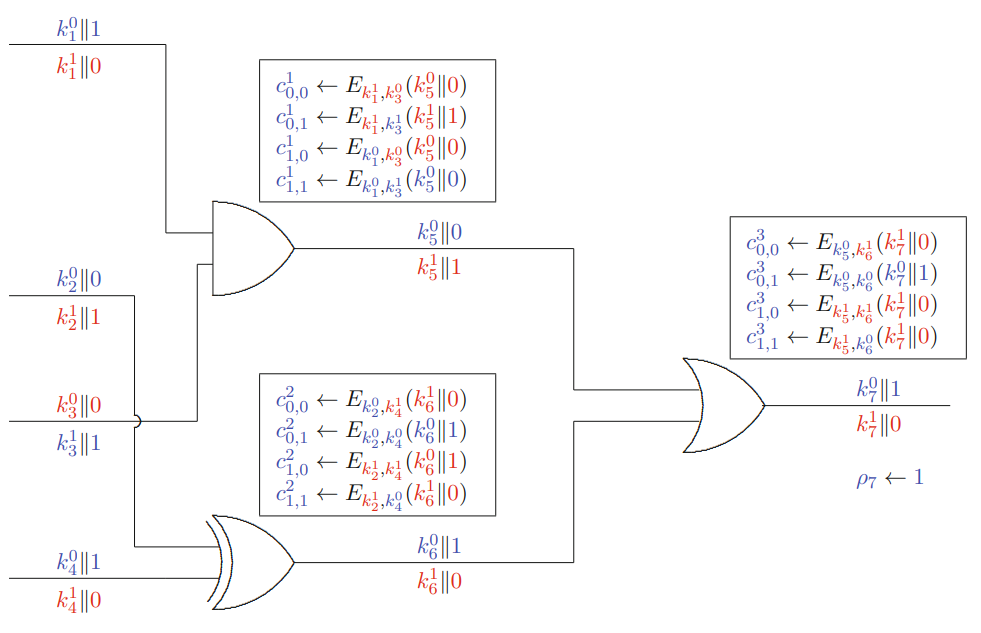
\includegraphics[width=0.8\linewidth]{garbled_valuation.png}
    \caption{Evaluacija šifrovanog kola za $f(\{w_1,w_2\},\{w_3,w_4\})=(w_1\land w_3)\lor(w_2\oplus w_4)$.}
\end{figure}
\end{frame}

% ---------------- JAOS PROTOCOL ----------------
\begin{frame}{Jaov protokol}
\begin{pblock}{Jaov protokol}
    \begin{enumerate}
        \item Učesnik $A$ konstruiše šifrovano kolo i $B$-u šalje samo vrednosti $c_{a,b}^i$.
        \item Učesnik $A$ zatim šalje $B$-u šifrovane vrednosti komponenti svojih ulaznih žica. 
        \item Učesnici $A$ i $B$ zatim izvršavaju protokol ignorantnog prenosa (engl. \textit{oblivious transfer, OT}) za svaku ulaznu žicu učesnika $B$. Cilj ovog koraka je da učesnik $B$ dobije tačno jedan od dva ključa koji odgovaraju njegovoj ulaznoj vrednosti, pri čemu učesnik $A$ ne saznaje koji je ključ izabran, dok učesnik $B$ ne dobija informaciju o drugom ključu.
        \item Učesnik $A$ zatim šalje $B$-u vrednosti $\rho_i$ za sve izlazne žice.
        \item Učesnik $B$ evaluira kolo koristeći šifrovane vrednosti ulaznih žica koje je dobio.
    \end{enumerate}
\end{pblock}
\end{frame}

\section{Slučaj više učesnika}
% ---------------- MULTI PARTY ----------------
\begin{frame}{Više učesnika: osnovna ideja}
\begin{itemize}
    \item Svaki učesnik poseduje privatni ulaz $x_i$
    \item Funkcija se predstavlja kao aritmetičko kolo
    \item Operacije nad kolom izvode se nad deljenim vrednostima
    \item Koristi se Šamirova (eng. \textit{Shamir's}) šema deljenja tajni
    \item Tajna $s$ predstavlja se kao konstantni član polinoma
    \[
    f(X)=s+a_1X+\cdots+a_tX^t
    \]
    
    \item Svaki učesnik dobija jednu evaluaciju:
    \[
    s^{(i)}=f(i)
    \]

    \item Bilo kojih $t+1$ učesnika može rekonstruisati tajnu (npr. Lagranžova interpolacija)
    \item Nijedan učesnik ne vidi kompletne ulaze drugih učesnika
\end{itemize}

\end{frame}

% ---------------- ARITHMETIC CIRCUITS ----------------
\begin{frame}{Aritmetička kola}
\begin{itemize}
    \item Čvorovi predstavljaju sabiračke i množačke kapije
    \item Sve operacije izvršavaju se nad konačnim poljem $\mathbb{F}_p$
    \item Ulazi i izlazi kapija predstavljaju vrednosti žica
    \item Složene funkcije mogu se predstaviti kombinacijom sabiranja i množenja
    \item Svaki učesnik kreira deljenja za svoje ulaze
\end{itemize}

\begin{figure}
    \centering
    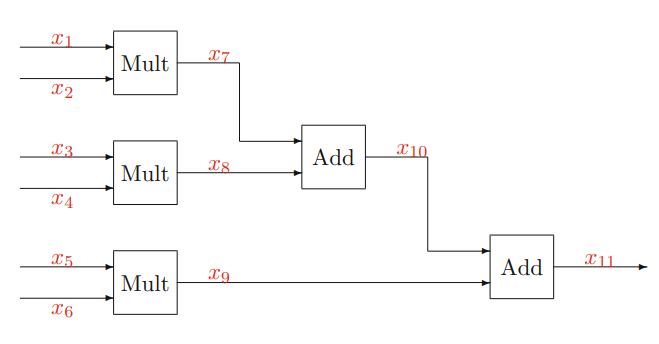
\includegraphics[width=0.65\linewidth]{arithmetic_circuit.png}
    \caption{Aritmetičko kolo za funkciju $f(x_1,\ldots,x_6)=x_1x_2+x_3x_4+x_5x_6$.}
\end{figure}

\end{frame}

% ---------------- ADDITION ----------------
\begin{frame}{Sabiranje deljenih vrednosti}
Pretpostavimo da su:

\[
a=f(0), \qquad b=g(0)
\]

deljeni pomoću polinoma stepena $t$.

\[
h(X)=f(X)+g(X)
\]

Tada važi:

\[
h(0)=a+b
\]

Svaki učesnik lokalno računa:

\[
c^{(i)}=a^{(i)}+b^{(i)}
\]

\begin{itemize}
    \item Nema komunikacije između učesnika
    \item Stepen polinoma ostaje isti
    \item Dobija se validno deljenje sume
\end{itemize}

\end{frame}

% ---------------- MULTIPLICATION ----------------
\begin{frame}{Množenje deljenih vrednosti}

Za razliku od sabiranja, množenje nije moguće izvesti samo lokalnim operacijama.

Ako svaki učesnik izračuna

\[
d^{(i)}=a^{(i)}b^{(i)},
\]

dobija se deljenje zasnovano na polinomu stepena $2t$ jer važi

\[
\deg(fg)=2t.
\]

\begin{itemize}
    \item Stepen polinoma se povećava
    \item Dobijeno deljenje više nije kompatibilno sa originalnom šemom
    \item Potrebno je izvršiti rekonstrukciju i ponovno deljenje rezultata
    \item Za rekonstrukciju se koriste Lagranžova interpolacija i koeficijenti rekombinacije
\end{itemize}

\end{frame}

\begin{frame}{MPC množenje}

\begin{enumerate}
    \item Svaki učesnik lokalno računa „privremeni proizvod“
    \[
    d^{(i)} = a^{(i)} b^{(i)}
    \]

    \item Svaki $d^{(i)}$ se ponovo deli Šamirovom šemom:
    \[
    \delta_i(0)=d^{(i)}, \quad \delta_i(j)=d_{i,j}
    \]

    \item Svaki učesnik $j$ dobija skup vrednosti:
    \[
    d_{1,j}, d_{2,j}, \ldots, d_{n,j}
    \]

    \item Rekombinacijom se formira novo deljenje:
    \[
    c^{(j)} = \sum_{i=1}^{n} r_i \, d_{i,j} \quad c = a \cdot b
    \]
\end{enumerate}

\begin{itemize}
    \item Lokalni proizvodi se ne koriste direktno kao tajna
    \item Kroz rekombinaciju se dobija validno Šamirovo deljenje proizvoda
    \item Rezultat ostaje skriven u polinomskom obliku
\end{itemize}

\end{frame}

% ---------------- HONEST BUT CURIOUS MODELS ----------------
\begin{frame}{Iskreni ali radoznali model}
\begin{itemize}
    \item Učesnici poštuju protokol
    \item Pokušavaju da izvuku dodatne informacije iz dostupnih podataka
    \item Privatnost se zasniva na Šamirovoj šemi deljenja tajni
\end{itemize}

Ako je broj korumpiranih učesnika:

\[
\le t
\]

tajna ostaje potpuno zaštićena.

Ako je broj korumpiranih učesnika:

\[
> t
\]

mogu rekonstruisati deljene vrednosti.

\end{frame}

% ---------------- MALICIOUS MODEL ----------------
\begin{frame}{Zlonamerni učesnici: problem}

U prethodnom modelu pretpostavlja se korektno izvršavanje protokola.

Zlonamerni učesnik može:

\begin{itemize}
    \item slati proizvoljne delove tajni
    \item manipulisati porukama u komunikaciji
    \item izazvati pogrešan izlaz MPC protokola
\end{itemize}

Posebno kritično:

\begin{itemize}
    \item MPC množenje zavisi od razmenjenih vrednosti
    \item jedna pogrešna poruka može pokvariti globalni rezultat
\end{itemize}

\end{frame}

% ---------------- MALICIOUS SOLUTION ----------------
\begin{frame}{Rešenje: priprema i glavna faza}

Protokol se deli u dve faze:

\begin{itemize}
    \item \textbf{Faza pripreme}: nezavisna od ulaza
    \item \textbf{Glavna faza}: evaluacija aritmetičkog kola
\end{itemize}

\textbf{Biverove (eng. \textit{Beaver's}) trojke u fazi pripreme:}
\begin{itemize}
    \item unapred se generišu deljene nasumične vrednosti $(a,b,c)$ gde je $c=a\cdot b$
    \item služe kao “referentni uzorak” za svako množenje u kolu
\end{itemize}

\textbf{Glavna faza:}
\begin{itemize}
    \item stvarno množenje se svodi na maskirane vrednosti $d=x-a$, $e=y-b$
    \item time se izbegava direktno operisanje nad privatnim vrednostima
    \item pogrešne ili nekonzistentne poruke se ne mogu neprimetno propagirati kroz kolo
\end{itemize}

\textbf{Bezbednost:}
\begin{itemize}
    \item proizilazi iz Šamirovog deljenja i ograničenja $t < n/3$
    \item omogućava detekciju nekonzistentnosti i sprečava uticaj zlonamernih učesnika na krajnji rezultat
\end{itemize}

\end{frame}


\standout{Pitanja?}

\standout{Hvala na pažnji!}

\end{document}


